\documentclass[conference]{IEEEtran}
\IEEEoverridecommandlockouts
% The preceding line is only needed to identify funding in the first footnote. If that is unneeded, please comment it out.
\usepackage{cite}
\usepackage{amsmath,amssymb,amsfonts}
\usepackage{algorithmic}
\usepackage{graphicx}
\usepackage{textcomp}
\usepackage{xcolor}
\def\BibTeX{{\rm B\kern-.05em{\sc i\kern-.025em b}\kern-.08em
    T\kern-.1667em\lower.7ex\hbox{E}\kern-.125emX}}
\begin{document}

\title{Brasil Sem Fake\\
}

\author{\IEEEauthorblockN{Gabriel A. M. de Sá}
\IEEEauthorblockA{\textit{dept. name of organization (of Aff.)} \\
\textit{name of organization (of Aff.)}\\
Brasília, Brasil \\
gabriel.sa@iesb.edu.br}
\and
\IEEEauthorblockN{Daniel L. O. Lucena}
\IEEEauthorblockA{\textit{dept. name of organization (of Aff.)} \\
\textit{name of organization (of Aff.)}\\
Brasília, Brasil \\
daniel.lucena@iesb.edu.br}
\and
\IEEEauthorblockN{Eduardo C. P. Fernandes}
\IEEEauthorblockA{\textit{dept. name of organization (of Aff.)} \\
\textit{name of organization (of Aff.)}\\
Brasília, Brasil \\
eduardo.fernandes@iesb.edu.br}
\and
\IEEEauthorblockN{Alan M. Nascimento}
\IEEEauthorblockA{\textit{dept. name of organization (of Aff.)} \\
\textit{name of organization (of Aff.)}\\
Brasília, Brasil \\
alan.nascimento@iesb.edu.br}
}

\maketitle

\begin{abstract}
O combate à desinformação vem se tornando um tópico de extrema importância. No contexto atual, a disseminação de notícias falsas ocorre em grande velocidade, onde redes sociais contribuem a este rápido alastramento. Muitas vezes estas notícias mimetizam a forma como notícias são tradicionalmente escritas, tornando o processo de detecção árduo e extenuante. Levando em consideração a dificuldade em categorizar tais notícias como fidedignas ou não de forma manual, esforços para a detecção automática destas estão sendo constantemente realizados. Neste artigo, será feito a investigação de quais características podem ser utilizadas ao treinar um classificador a fim de obter maior acurácia. Além disso, como a atual dificuldade em encontrar e criar datasets rotulados na língua portuguesa afeta o treinamento destes classificadores.
\end{abstract}

\begin{IEEEkeywords}
NLP, fake news, características
\end{IEEEkeywords}

\section{Introduction}
Caracterizada como notícias falsas que são compartilhadas deliberadamente com a intenção de enganar o leitor, as notícias falsas (Frequentemente chamadas de fake news) são uma grande ameaça. De acordo com um estudo feito em 2017 \cite{b1}, foi possível verificar que havia uma quantidade maior de fake news que favoreciam o canditato à presidência Doanld Trump quando comparado com as compartilhadas em favor da Hillary Clinton, outra candidata ao cargo. Este fenômeno não é exclusivo ao Estados Unidos, posto que também foi observado, ao ser feito a análise de 346 notícias falsas \cite{b2} compartilhadas durante o periodo eleitoral em 2018, que 45\% dessas eram diretamente favoráveis ao candidato Jair Bolsonaro, que eventualmente foi eleito como presidente.

Ao observar este fenômeno, torna-se claro o impacto das notícias falsas na política. Enquanto este é um exemplo pertinente, suas consequências vão além deste meio, afetando até mesmo a área da saúde. Em notícias, o presidente Jair Bolsonaro defendia o uso da cloroquina e hidroxicloroquina como "tratamento precoce" para a covid-19, mesmo após a divulgação de evidências científicas que mostravam que estas não traziam benefícios aos pacientes que combatiam o vírus.

Ao entender o impacto que as fake news tem em diversos setores, podemos também ver porque a sua detecção é tão importante. Porém, para combater sua propagação, primeiro há a necessidade de detecta-las. Como há um volume grande de notícias circulando constantemente, não é conveniente dar o trabalho de verificar sua veracidade a uma pessoa, consequentemente, a detecção automática usando técnicas de Natural Language Processing (NLP) e Machine Learning podem suprir esta lacuna.

Para chegar ao resultado esperado, isto é, a detecção de fake news de forma automática baseada em NLP, deve ser definido quais características vão ser levadas em consideração para fazer o treinamento do algorítmo de machine learning escolhido. Em virtude disso, diferentes trabalhos que buscam o mesmo fim costumam diferir quanto a escolha de características. Tais trabalhos serão discutidos posteriormente, e também será feito um estudo com o objetivo de determinar quais conjuntos de características concluimos serem as mais pertinentes ao analisar as notícias, a fim de obter uma maior acurácia em sua detecção.


\section{Trabalhos correlatos}

Em seu artigo, Monteiro et al. \cite{b3} faz a análise das notícias utilizando como algorítmo de machine learning o support vector machine (SVM), e como características podemos citar algumas: A quantidade média de sentenças, verbos, adjetivos, advérbios, e além destes valores de quantidade, também é feita a análise de sentimentos. Para evitar algum tipo de viés, os resultados quantitativos foram analisados com base na quantidade total de tokens, posto que foi observado que as notícias verdadeiras eram, em sua maioria, bem maiores que as notícias falsas. É importante ressaltar que este artigo é o único citado neste trabalho que utiliza as notícias com língua portuguesa, além de ter realizado a criação de uma corpus com mais de 7000 notícias, todas categorizadas, na chamada fake.br corpus.

Enquanto existem sites dedicados a exposição de notícias falsas (Como o \url{https://www.boatos.org}), a obtenção destas ainda se mostra um desafio, especialmente num contexto em que datasets vastos são um requisito na composição de um classificador confiável. Então, Hauch et al. \cite{b4} fala sobre como a maioria das descobertas na área foram feitas em inglês, além de trazer a tona um importante detalhe: Línguas diferentes apresentam caracteristicas diferentes que devem ser levadas em conta. Com isso, além das diferenças culturais, apenas realizar a tradução de notícias feitas em outra língua para obter uma maior quantidade de dados se mostra inviável. Hauch et al. também traz algumas características interessantes, e.g. causa, onde é feita a verificação da porcentagem de palavras que buscam atribuir causa ao que quer que esteja sendo descrito, também a certitude, como palavras do tipo "porque" e "nunca".

Em sua pesquisa, Rashkin et al. \cite{b5} divide as notícias em três grupos: Sátira, Hoax (Farsas) e propaganda (Em que engana o leitor em prol de uma agenda política). Sátiras também mimetizam notícias verdadeiras, porém costumam apresentar deixas que mostram que não devem ser levadas a sério. Em virtude disso, neste trabalho, serão ignoradas as notícias de natureza satírica. Já em seus resultados, Rashkin et al. afirma que palavras podem ser usadas para exagerar algo, como superlativos e advérbios modais, são utilizadas com maior frequência em notícias falsas, já palavras que indicam valores concretos, como comparativos e números, estavam mais presentes em notícias verdadeiras.

\section{Tratamento do texto}
Para realização da extração das características de um texto, antes foi realizado uma série de etapas que buscam normalizar sua estrutura, isto é, é feita a remoção de elementos considerados dispensáveis, e muitas vezes, prejudiciais para o processamento de um computador, a fim da criação de uma matriz de termo de documento (document-term matrix), e posteriormente o ato de inferir dela os dados que julgamos relevantes.

\subsection{Remoção das pontuações}\label{AA}
Inicialmente, são realizadas algumas técnicas que buscam garantir que todas as palavras não contenham caracteres especiais e afins. Primeiro, são substituidos todos os caracteres maiúsculos por minúsculos, e então é feita a remoção de todas as pontuações e dígitos do texto.

\begin{figure}[htbp]
\centerline{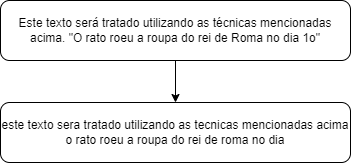
\includegraphics[scale=0.5]{figura1.png}}
\caption{Primeira etapa de limpeza}
\label{fig}
\end{figure}

Este passo é importante para garantir que não ocorram problemas como a definiçaõ de "também" e "tambem" como duas palavras diferentes.


\subsection{Remoção de stopwords}
Agora, o próximo passo servirá para que não haja a presença de stopwords (palavras irrelevantes), isto é, palavras que não estão contribuindo para o entendimento da informação principal apresentada no texto. Estas palavras aparecem em abundância em qualquer linguagem humana, e para chegar a uma lista que abrange o máximo de stopwords foram realizadas etapas de análise exploratória das notícias, além da busca em bibliotecas que forneciam esses dados (E.G. NLTK \cite{b6})

\begin{figure}[htbp]
\centerline{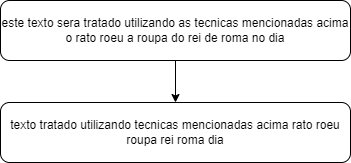
\includegraphics[scale=0.5]{figura2.png}}
\caption{Remoção das stopwords do texto}
\label{fig}
\end{figure}

\subsection{Lemming}
Finalmente, será aplicada a técnica de lemming, ou seja, as palavrãs serão reduzidas a sua raiz, o lemma. 

\begin{figure}[htbp]
\centerline{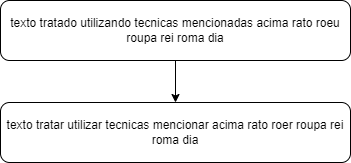
\includegraphics[scale=0.5]{figura3.png}}
\caption{Remoção das stopwords do texto}
\label{fig}
\end{figure}

Ao decidir se seria feito o stemming ou lemming, foi levada em conta que a prioridade é reduzir as palavras a outras que também são gramaticalmente correta, a fim de evitar problemas como stems que foram cortados demais e resultaram numa palavra que não tem mais sentido, ou palavras que apresentavam significados diferentes mas foram reduzidas ao mesmo stem. 

\section{Características a serem analisadas}

Com o texto devidamente tratado e organizado numa document-term matrix, resta fazer a análise das características que desejamos, para posteriormente serem usadas para o treinamento de um classificador. Tomando em consideração trabalhos corretos, foram levadas em consta quais características foram comumente utilizadas \cite{b7} para então definir quais serão exploradas neste trabalho.

Como esperado, a atual seleção varia em seus tipos, citando algumas: Temos quantificadores (e.g. Quantidade de caracteres), verificações da complexidade das frases (e.g. Média de palavras por frase), análise de sentimentos (e.g. \% de palavras positivas). O objetivo desta seleção é cobrir uma variedade grande de tipos, e então, combina-los a fim de encontrar quais uniões resultarão na melhor acurácia.

Por fim, será feita também a investigação das consequências que a atual carência de datasets rotulados e amplos traz para o treinamento de algorítmos classificadores, especificamente na lingua portuguesa.

\begin{figure}[htbp]
\centerline{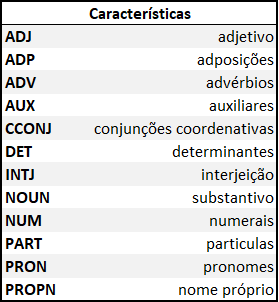
\includegraphics[scale=0.5]{tabela1.png}}
\caption{Tabela com características}
\label{fig}
\end{figure}

\section{Resultados esperados}
Em virtude das limitações impostas pelo dataset, um resultado possível é o overfitting. Basicamente, a obtenção de notícias atuais se mostra um fator importante, posto que os assuntos abordados nelas podem variar dramaticamente em um curto período \cite{b7}. Levando isso em conta, e o fato de que a maior corpus publicada em português conta com apenas 7200 notícias já categorizadas, o primeiro desafio se encontra já na coleta de notícias.

Além disso, utilizaremos a precisão como principal métrica de avaliação, pois no contexto atual, notícias falsas que são categorizadas erroneamente como verdadeiras acabam sendo mais prejudiciais do que o contrário. A partir disso, escolheremos as características que mais se adequam com o propósito de evitar estes falsos positivos.


\begin{thebibliography}{00}
\bibitem{b1} Allcott, Hunt, and Matthew Gentzkow. 2017. "Social Media and Fake News in the 2016 Election." Journal of Economic Perspectives, 31 (2): 211-36.
\bibitem{b2} T. M. S. Galvão, "Fake News na eleição presidencial de 2018 no Brasil", tese, doutorado, comunicação e cultura contemporâneas, UFBA
CONTEMPORÂNEAS, 2020
\bibitem{b3} Monteiro, R.A.; Santos, R.L.; Pardo, T.A.; de Almeida, T.A.; Ruiz, E.E.; Vale, O.A. Contributions to the Study of Fake News in
Portuguese: New Corpus and Automatic Detection Results. In International Conference on Computational Processing of the Portuguese
Language; Springer: Berlin, Germany, 2018; pp. 324–334.
\bibitem{b4} Hauch, V.; Blandón-Gitlin, I.; Masip, J.; Sporer, S.L. Are computers effective lie detectors? A meta-analysis of linguistic cues to
deception. Personal. Soc. Psychol. Rev. 2015, 19, 307–342.
\bibitem{b5} Rashkin, H.; Choi, E.; Jang, J.Y.; Volkova, S.; Choi, Y. Truth of varying shades: Analyzing language in fake news and political
fact-checking. In Proceedings of the Conference on Empirical Methods in Natural Language Processing, Copenhagen, Denmark,
9–11 September 2017; pp. 2931–2937.
\bibitem{b6} S. Bird, Natural language processing with python. O'Reilly Media, 2016. 
\bibitem{b7} N. R. de Oliveira, P. S. Pisa, M. A. Lopez, D. S. V. de Medeiros, and D. M. F. Mattos, “Identifying Fake News on Social Networks Based on Natural Language Processing: Trends and Challenges,” Information, vol. 12, no. 1, p. 38, Jan. 2021, doi: 10.3390/info12010038.
\end{thebibliography}
\vspace{12pt}
\color{red}


\end{document}
